\documentclass{standalone}

\usepackage{tikz}
\usetikzlibrary{calc}

\def\sep{0.2}

\def\scalefact{4}
\def\scalerad{\scalefact*1pt}
\begin{document}
  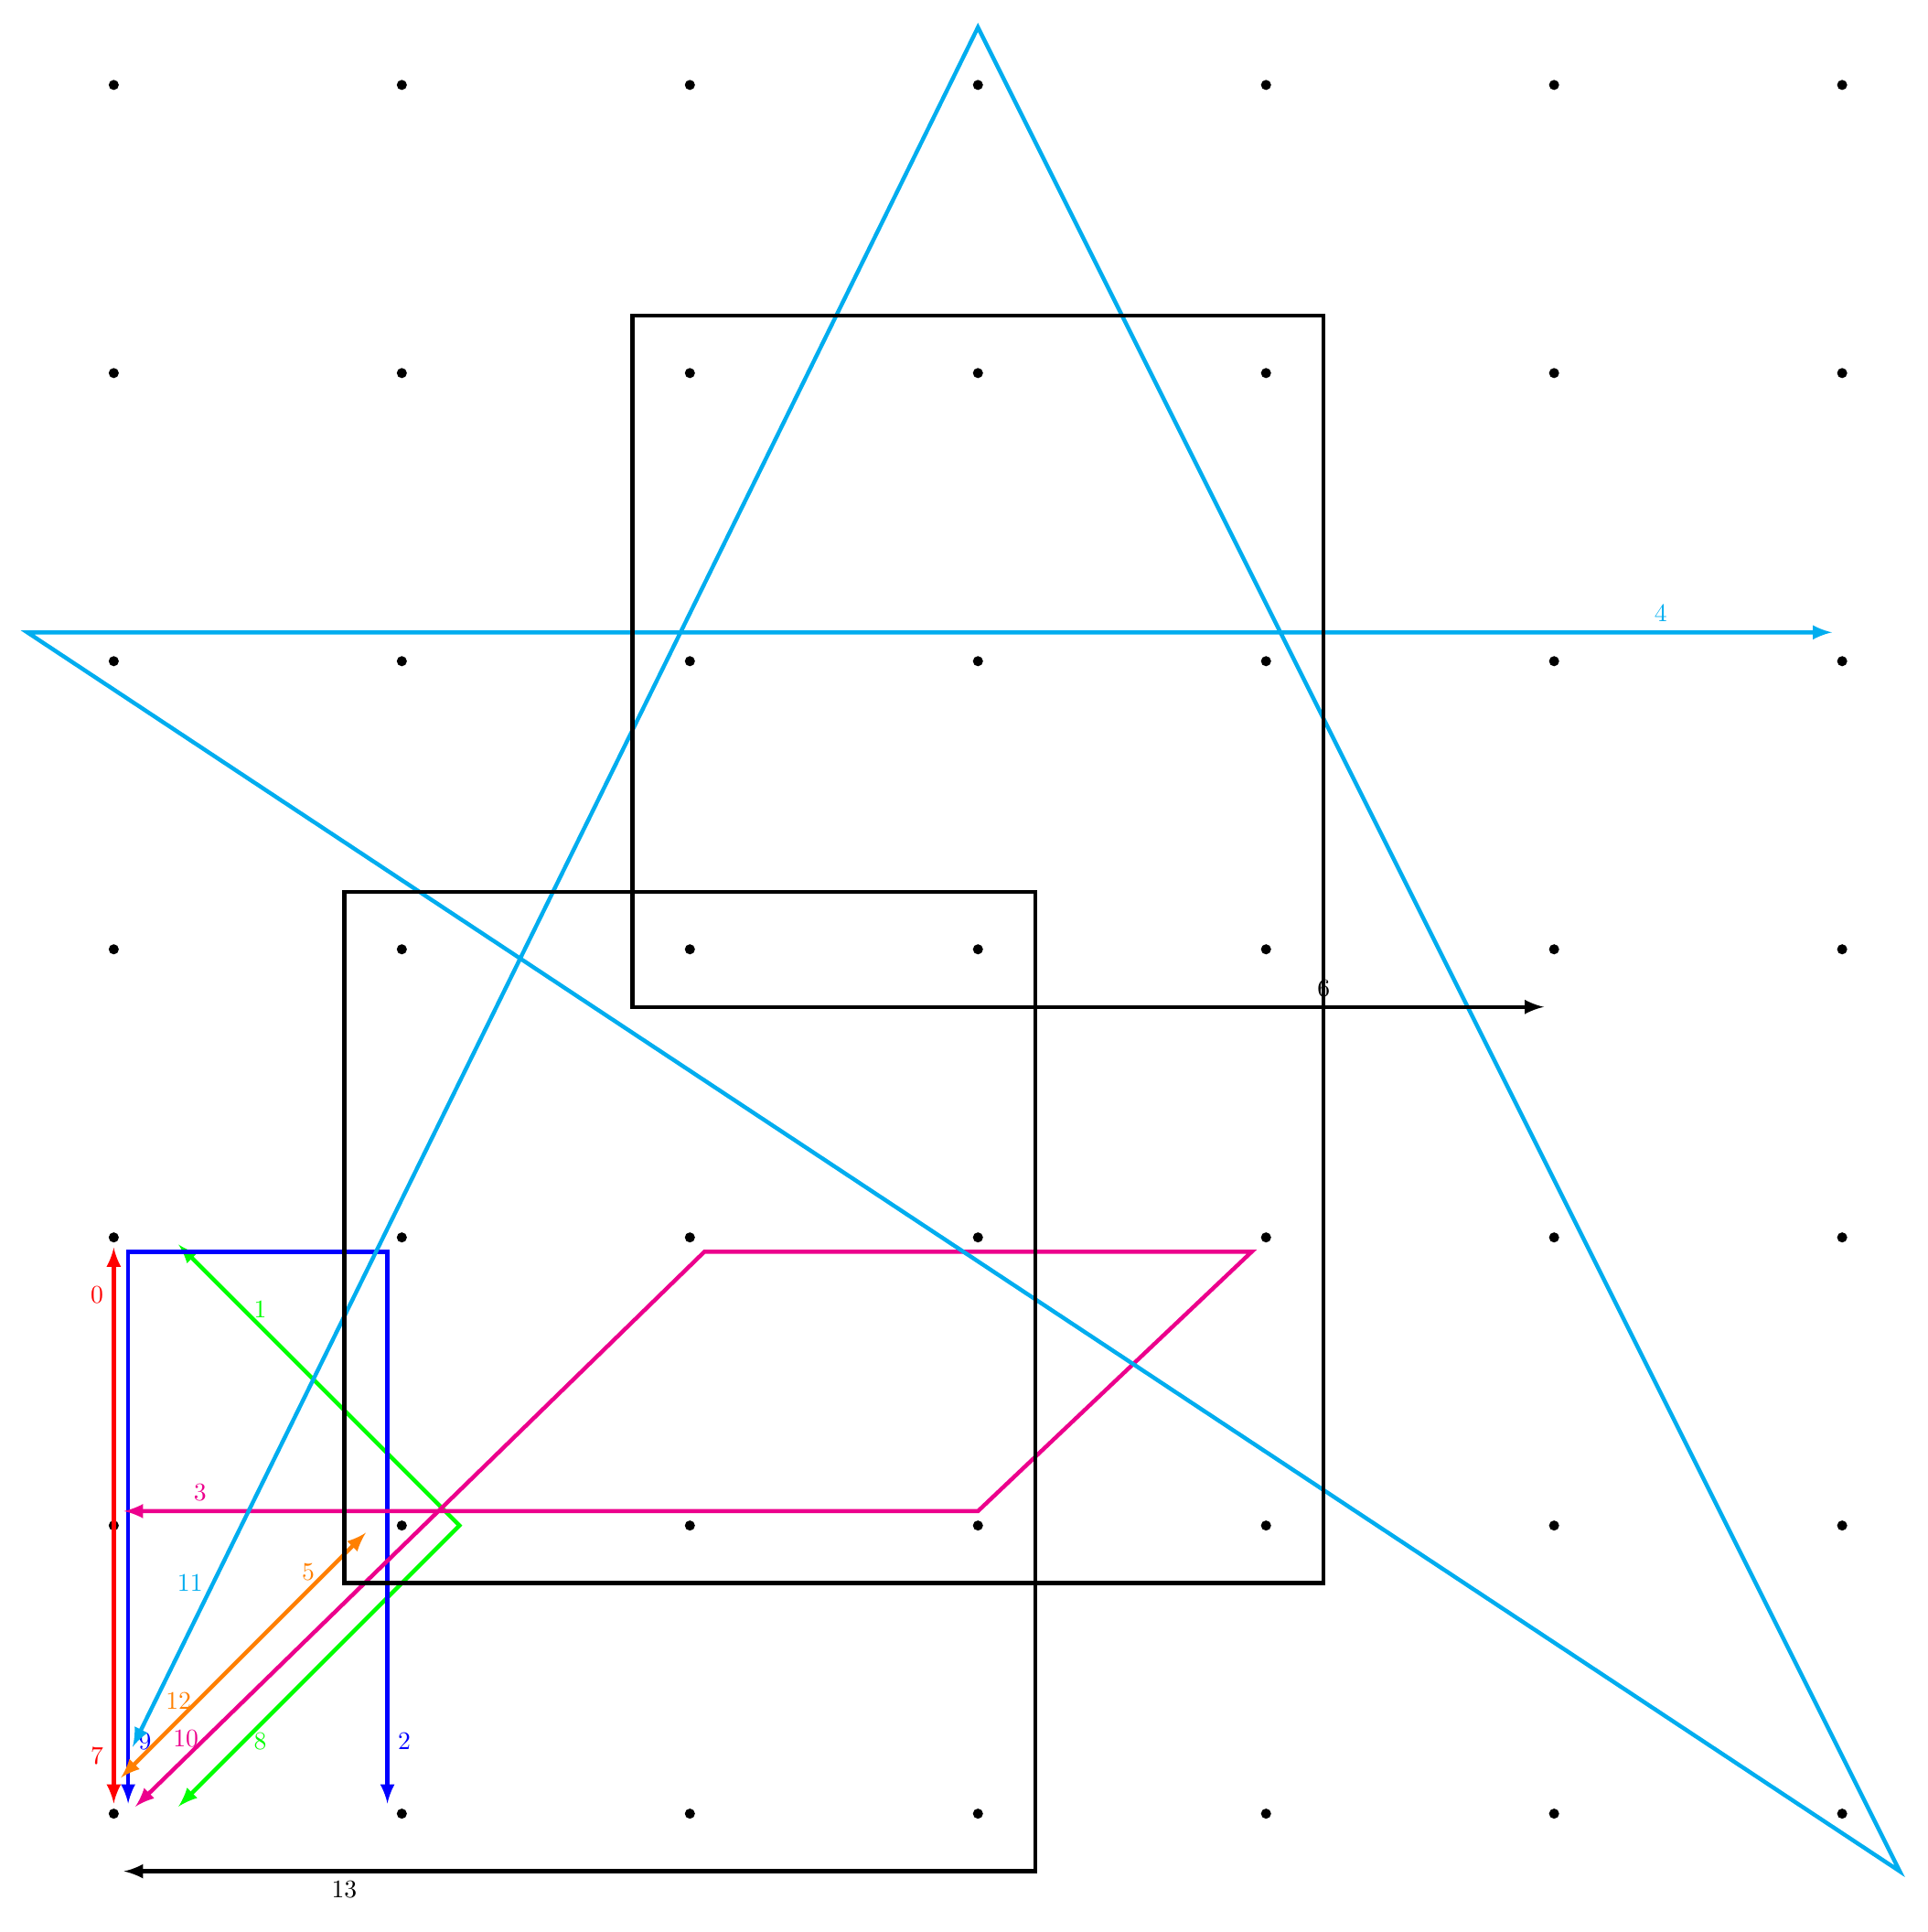
\begin{tikzpicture}
    \tikzset{%
      polyline/.style={%
        ultra thick, latex-latex, shorten <= \scalerad, shorten >= \scalerad}}

   % \draw[help lines,step=\scalefact] (0,0) grid ($(4*\scalefact ,2*\scalefact)$);
    \foreach \i in {0,1,2,3,4,5,6}
    \foreach \j in {0,1,2,3,4,5,6}{
      \coordinate (p\i\j) at ($(\scalefact*\i,\scalefact*\j)$);
      \fill (p\i\j) circle (0.5*\scalerad);
    }

    \draw[polyline,red] (p00) -- node[pos=0.2, left]{7} (p01) -- node[pos=0.8, left]{0}(p02);

    \draw[polyline,green] ($(p00)+(4*\sep,0)$) -- node[near start, right]{8} ($(p11)+(4*\sep,0)$) -- ($(p02)+(4*\sep,0)$) node[near end, right]{1};

    \draw[polyline,blue] ($(p00)+(\sep,0)$) -- node[near start, right]{9} ($(p01)+(\sep,0)$) -- ($(p02)+(\sep,-\sep)$) -- ($(p12)+(-\sep,-\sep)$) -- ($(p11)+(-\sep,0)$) -- node[near end, right]{2} ($(p10)+(-\sep,0)$);

    \draw[polyline,magenta] ($(p00)+(\sep,0)$) -- node[pos=0.1, above]{10} ($(p22)+(\sep,-\sep)$) -- ($(p42)+(-\sep,-\sep)$) -- ($(p31)+(0,\sep)$) -- node[pos=0.9, above]{3} ($(p01)+(0,\sep)$);

    \draw[polyline,cyan] ($(p00)+(\sep,4*\sep)$) -- node[pos=0.1, left]{11} ($(p36)+(0,4*\sep)$) -- ($(p60)+(4*\sep,-4*\sep)$) -- ($(p04)+(-6*\sep,2*\sep)$) -- node[pos=0.9, above]{4} ($(p64)+(0,2*\sep)$);

    \draw[polyline,orange] ($(p00)+(0,2*\sep)$) to node[near start,above]{12} node[near end, above]{5} ($(p11)+(-2*\sep,0)$);

    \draw[polyline,black] ($(p00)+(0,-4*\sep)$) -- node[near start,below]{13} ($(p30)+(4*\sep,-4*\sep)$) -- ($(p33)+(4*\sep,4*\sep)$) -- ($(p13)+(-4*\sep,4*\sep)$) -- ($(p11)+(-4*\sep,-4*\sep)$) -- ($(p41)+(4*\sep,-4*\sep)$) -- ($(p45)+(4*\sep,4*\sep)$) -- ($(p25)+(-4*\sep,4*\sep)$) -- ($(p23)+(-4*\sep,-4*\sep)$) -- node[near end, above]{6} ($(p53)+(0,-4*\sep)$);
  \end{tikzpicture}
\end{document}

%%% Local Variables:
%%% mode: latex
%%% TeX-master: t
%%% End:
